%! TeX program = xelatex
%! TEX-TS program = xelatex
\documentclass[aspectratio=169,xcolor={dvipsnames}]{beamer}

\input{/home/shiroha/Documents/latex/templates/slides/metro_lm.tex}

% % references
% \setbeamertemplate{bibliography item}[text] % change reference icon to number
% \setbeamertemplate{frametitle continuation}{} % remove 'i' before frametitle 'Reference'
% \usepackage[backend=biber,style=chem-acs]{biblatex}
% \usepackage{bibentry} % enable direct bibentry print
% \addbibresource{references.bib}


% title page
\newcommand\mail{has015@ucsd.edu}
\title{CHEM 6B WI24 F02-F06}
\subtitle{Week 2: kinetic-molecular theory of gases} 
\author{TA: Haoran Sun (\href{mailto:\mail}{\mail})}
\institute{University of California, San Diego}
\date{January 19, 2024}

\begin{document}

\maketitle

% \begin{frame}{Outline}
%     \tableofcontents
% \end{frame}


\begin{frame}[t]
    \frametitle{Statistics: mean}
    \begin{itemize}
        \item Average of a data set $x_i$/probability distribution $p(x_i)$
            (discrete) or $f(x)$ where
            $x$ lives in $[a, b]$ (continuous)
            is defined as 
            \begin{align}
                x_\text{mean} &= \frac{1}{N}\sum_i x_i \text{ or }
                \sum_i x_ip(x_i)\text{ or }
                \int_a^b xf(x)\d x
            \end{align}
            where $N$ is the size of the dataset (discrete).
        \item Example: given a set of numbers
            \begin{align*}
                1, 1, 3, 3, 3, 4
            \end{align*}
            Calculate the mean of this dataset.
    \end{itemize}
\end{frame}

\begin{frame}[t]
    \frametitle{Statistics: mean square \& root mean square}
    \begin{itemize}
        \item Mean square is the mean of square
            \begin{align}
                x_\text{ms} &= \frac{1}{N}\sum_i x_i^2 \text{ or }
                \sum_i x_i^2 p(x_i)\text{ or }
                \int_a^b x^2f(x)\d x
            \end{align}
        \item Example: given a set of numbers
            \begin{align*}
                1, 1, 3, 3, 3, 4
            \end{align*}
            Calculate the root mean square of this dataset.
    \end{itemize}
\end{frame}

\begin{frame}[t]
    \frametitle{Statistics: mode}
    \begin{itemize}
        \item Mode is the value in the dataset which gives the maximum probability
            (i.e., the most probable value)
            \begin{align}
                x_\text{mp} &= \sum_i \argmax_{x_i} p(x_i) \text{ or }
                \argmax_x f(x)
            \end{align}
        \item Example: given a set of numbers
            \begin{align*}
                1, 1, 3, 3, 3, 4
            \end{align*}
            Calculate the mode of this dataset.
    \end{itemize}
\end{frame}


\pgfmathdeclarefunction{maxwell}{2}{%
  \pgfmathparse{4/sqrt(pi)*(\k/#2)^(3/2)*(#1^2)*exp(-\k*(#1^2)/#2)}%
}
\def\maxwell#1#2{4/sqrt(pi)*(\k/#2)^(3/2)*((\xscale*#1)^2)*exp(-((\xscale*#1)^2)*(\k/#2))}
%\def\vmax#1{sqrt(#1/\k)/\xscale}
\def\tick#1#2{\draw[thick] (#1) ++ (#2:0.03*\ymax) --++ (#2-180:0.06*\ymax)}
\begin{frame}[t]
    \frametitle{Kinetic theory of gas}
    \begin{itemize}
        \item Three essential statistical values for gas.
            $v_\text{mp}$: most probable. 
            $v_\text{mean}$: average. 
            $v_\text{rms}$: root-mean-square.
            \begin{align}
                v_\text{mp} &= \sqrt{\frac{2RT}{M}},\quad
                v_\text{mean} = \sqrt{\frac{8RT}{\pi M}},\quad
                v_\text{rms}  = \sqrt{\frac{3RT}{M}}
            \end{align}
        \item $v_\text{mp} < v_\text{mean} < v_\text{rms}$.
    \end{itemize}
    \begin{figure}
        \centering
        \begin{tikzpicture}[scale=0.8]
          \def\xmax{6.0}
          \def\ymax{4.0}
          \def\k{4500} % k = m/2k
          \def\xscale{0.14}
          \def\vn{2.6}
          \def\vmax{sqrt(300/\k)/\xscale}
          \def\vrms{sqrt(300/(2*\k/3))/\xscale}
          \def\vave{2*\vmax/sqrt(pi)}
          \coordinate (O) at (0,0);
          \coordinate (X) at (\xmax,0);
          \coordinate (Y) at (0,\ymax);
          
          % AXIS
          \draw[<->,thick]
            (Y) node[above left,rotate=90] {Probability} -- (0,0) -- (X) 
            node[right=4,below] {$v$ [\si{m/s}]};
          \foreach 
          %\x [evaluate={\c=sqrt(\k/0.00096); \v=(round(\x*\c/\xscale))}] in {1,...,3}{
                   \i [evaluate={\v=int(\i*200);}] in {0,...,5}{
            \pgfmathsetmacro\x{\v*sqrt(0.00192)/\xscale/sqrt(\k))} % higher precision
            \tick{\x,0}{90} node[below,scale=0.8] {\v};
          }
          
          \draw[dashed,thin]
            ({\vmax},0) coordinate (VM) --++ (0,{1.04*\maxwell{\vmax}{300}})
            node[left=1,above left=-4,scale=0.9] {$v_\text{mp}$};
          \draw[dashed,thin]
            ({\vave},0) coordinate (VA) --++ (0,{1.04*\maxwell{\vmax}{300}})
            node[right=1,above=0,scale=0.9] {$v_\text{mean}$};
          \draw[dashed,thin]
            ({\vrms},0) coordinate (VR) --++ (0,{1.04*\maxwell{\vmax}{300}})
            node[above=2,below right=0,scale=0.9] {$v_\text{rms}$};
          %\tick{VM}{90}; %node[myblue,right=1,below left=0,scale=0.85] {$v_\text{p}$};
          %\tick{VA}{90}; %node[myred,left=1,below=-2,scale=0.85] {$\expval{v}$};
          %\tick{VR}{90}; %node[mygreen,below right=0,scale=0.85] {$v_\text{rms}$};
          
          % PLOT
          \draw[blue!50!black,thick,samples=100,smooth,variable=\x,domain=0.01:0.94*\xmax]
            plot(\x,{\maxwell{\x}{300}});
          
        \end{tikzpicture}
    \end{figure}
\end{frame}

\begin{frame}[t]
    \frametitle{Problems}
    \begin{block}{Activity 1.1}
        Measurement on a noble gas sample at a temperature of $\SI{1000}{\kelvin}$
        show a discribution of molecular speeds characterized by a root mean square
        speed of $\SI{1.12e3}{\metre\second^{-1}}$.
        What noble gas is this?
    \end{block}
\end{frame}

\begin{frame}[t]
    \frametitle{Problems}
    \begin{columns}
    \begin{column}{.65\textwidth}
    \begin{block}{Activity 1.2}
        Consider two Maxwell-Boltzmann speed distribution curves below
        \begin{enumerate}[a.]
            \item If the curve represent the speed distributions for argon and 
                helium \ul{at the same temperature}, which curve
                (1 or 2) best depicts the behavior of helium?
            \item If the curves represent the speed distributions for helium gas
                \ul{at two different temperatures}, $T_1$ and $T_2$
                (where $T_2>T_1$), which curve (1 or 2) best depicts the hither
                temperature sample? 
        \end{enumerate}
    \end{block}
    \end{column}
    \begin{column}{.35\textwidth}
        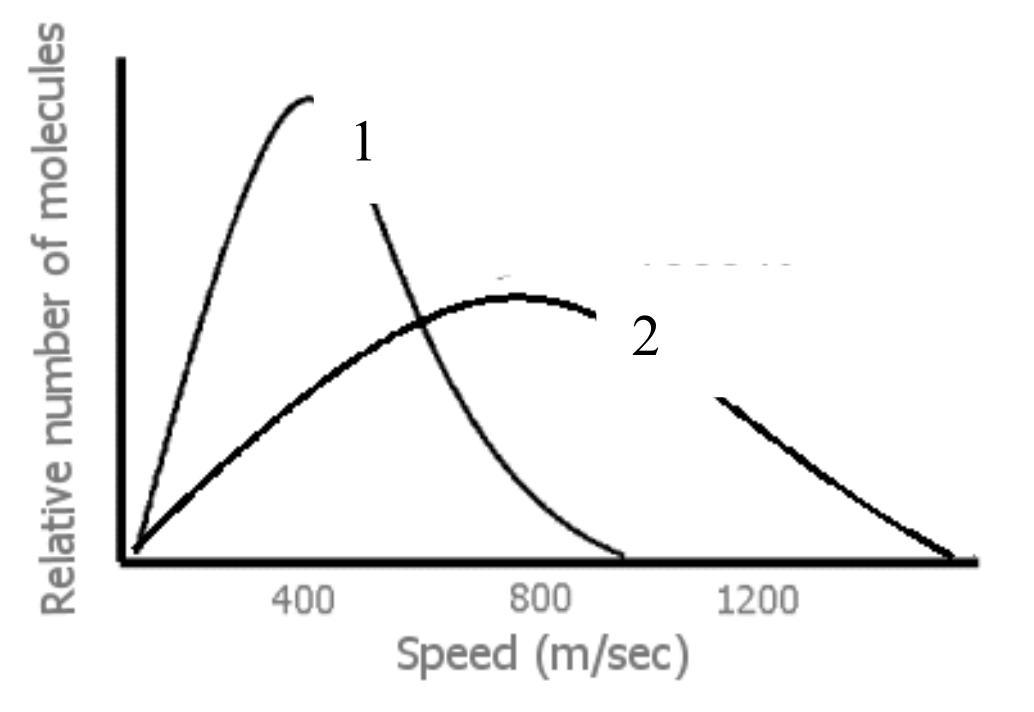
\includegraphics[width=\textwidth]{2b.png}
    \end{column}
    \end{columns}
\end{frame}


% % reference page
% \begin{frame}[allowframebreaks]
%     \frametitle{References}
%     \nocite{*}
%     \printbibliography
% \end{frame}

\end{document}



